\chapter{Discussion}
\section{Scope}
The results of our HRV analyses must be interpreted within the scope and limitations of this study. Most importantly, our analyses were designed to simulate vegetation dynamics under a historic reference period. We chose the period from 1550 to 1850, representing the 300 years prior to European settlement, based on expert opinion (Safford, pers. comm. 20 September 2013). The arrival of European settlers to the Sierra Nevada was spurred primarily but not exclusively by the Gold Rush, and led to sweeping ecological changes that now have greatly altered many Sierran landscapes -- through fire suppression, grazing, road-building, timber cutting, recreation, and other activities (Meyer 2013, Safford 2013, \todo{OTHERS}). Climatically, this time frame does fall during the ``Little Ice Age.'' However, Safford (2013) argues that vegetation change did not change substantially during the time. The period prior to European settlement, then, is a suitable reference condition against which we can compare current landscape structure and dynamics. Moreover, it is frequently used in the western United States as the historical reference period for restoration planning (Safford 2013). The period is also up to several times the length of rotation periods identified for well-understood cover types within the project area. Finally, it is a timeframe for which we have a reasonable amount of specific information to enable us to model the system.

We do not argue here that the chosen reference period was a time of stasis, climatically, ecologically, or culturally. In Figure \ref{pdsi} we illustrate how the Palmer Drought Severity index, a measure of climate variability, oscillates around an average value throughout the reference period. Multi-year droughts and El Niño/La Niña events also occurred over this time frame (Meyer 2013). Ecologically, our historical period occurred during a very long-term (on the scale of thousands of years) shift to a warmer and drier climate, with an associated shift toward species more tolerant of such conditions, such as yellow pine species, and away from species like white fir, which prefer more mesic conditions. A slow shift toward more frequent fire was also taking place (Safford 2013). Culturally, several Native American tribes were living throughout the project area during the reference period. Debate continues among scientists and researchers as to the extent to which those peoples managed vegetation through setting fires (Safford 2013, \todo{OTHERS}). Because we lack empirical evidence to distinguish between lightning-caused and human-caused fires during the reference period, we decided not to exclude any fire frequency or rotation data on the basis of not being reflective of ``natural'' conditions.

We emphasize that our choice of reference periods does not suggest that it should be our goal in management to recreate all of the ecological conditions and dynamics of this period. Complete achievement of such a goal would be impossible, given the climatic, cultural, and ecological changes that have occurred in the last century. It also would be unacceptable socially, economically, and politically. Nor do we suggest that the reference period was completely ``natural'' or preferable in all ways to today’s landscape. 

\begin{wrapfigure}{r}{0.5\textwidth}
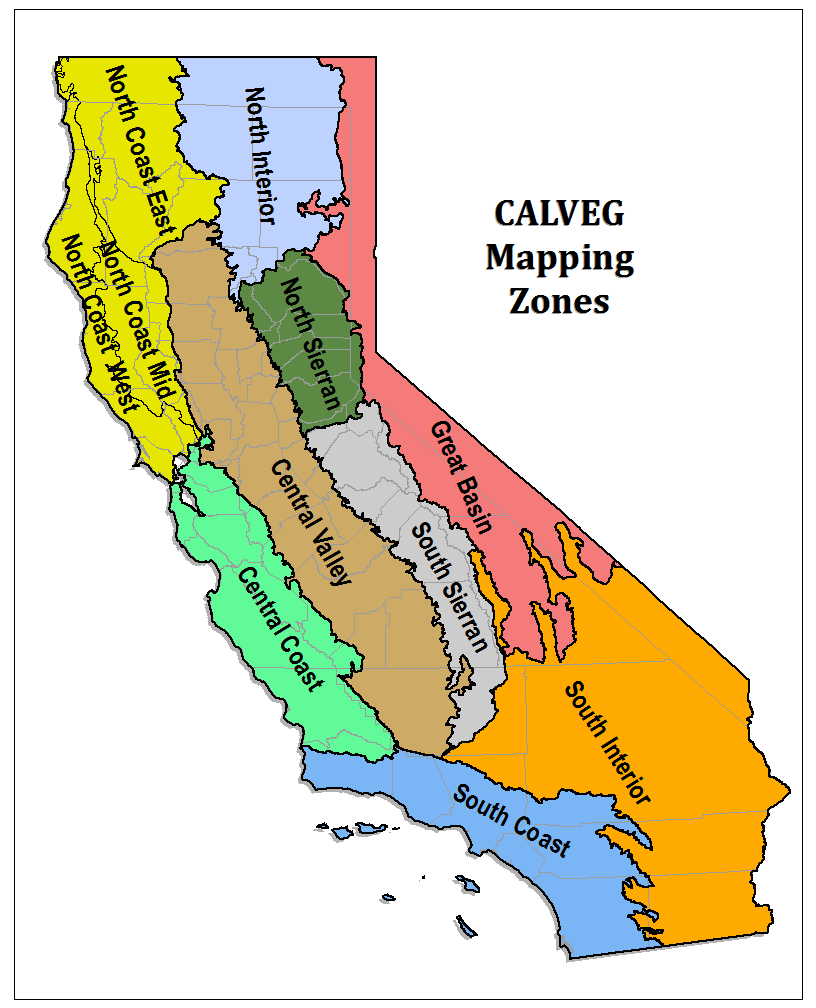
\includegraphics[width=0.48\textwidth]{images/CALVEGmappingzones.png}
\caption{\small CALVEG Mapping Zones. These zones meet U.S. Forest Service standard at national and regional levels. These ecological provinces are associated with dozens of vegetation alliances, which are used to classify vegetation in spatial data products.} 
\label{calveg}
\end{wrapfigure}

However, the reference period proposed will allow us to compare current conditions to a baseline set of data on ecosystem conditions (composition, configuration, and disturbance processes) ``to develop an idea of trend over time and idea of the level of depature of altered ecosystems from their ``natural'' state'' (Safford 2013). The results presented here will complement the Natural Range of Variability assessments compiled by the Forest Service's Pacific Southwest Region Ecology group \todo{cite}. An understanding of natural landscape structures and variability during this reference period also provides a basis for forest management policies and associated actions that seek to mimic natural disturbance patterns  (Romme et al. 2000, Buse and Perera 2002).

The spatial scope of our project extends generally to the the northern Sierra Nevada. When deciding on land cover types, including determining xeric and mesic subtypes, our focus was to best represent the project area and the surrounding landscape. We used the CALVEG Mapping Zone boundary for the ``North Sierra'' (Figure \ref{calveg}) as our focus for defining vegetation and disturbance, including susceptibility, response to fire, and fire size and distribution \todo{cite?}. The model could be applied, with some revision, to the east-side of the Sierra Nevada, or to the southern mountains.

\section{Limitations}

Because our study relied on the use of computer models, it is imperative that the limitations of these models be understood before applying the results in a management context. Here, we discuss several important limitations, some general to the modeling approach employed here and some specific to how we parameterized these models for application in the northern Sierra Nevada.

First, our approach relies heavily on the use of computer models, and while it is important to recognize the many advantages of models, it is critical to understand that models are abstract and simplified representations of reality. \textsc{RMLands}, in particular, simulates wildfires, but does not simulate all of the disturbance processes or all of the complex interactions among them that characterize real landscapes. Ultimately, the results of a model are constrained by the quality of input data. While \textsc{RMLands} utilizes a rich database, the data layers themselves are not perfect. For example, the vegetation cover layer is subject to human interpretation errors and objective classification errors, and is further limited by the spatial resolution of the grid. Thus, our results should not be interpreted as ``golden''. Rather, they should be used to help identify the most influential factors driving landscape change, critical empirical information needs, interesting system behavior, the limits of our understanding, a basis for exploring “what if” scenarios.

Second, it is important to realize that \textsc{RMLands} requires substantial parameterization before it can be applied to a particular landscape. To the extent possible, we have utilized local empirical data. However, we also drew on relevant scientific studies, often from other geographic locations, and relied heavily on expert opinion when scientific studies and local empirical data were not available. The source of information used to parameterize the models is fully documented and subject to review. Thus, our results should not be viewed as definitive, but rather as an informed estimate of the HRV based on our current scientific understanding. It is important to understand that our estimate of the HRV is subject to change as new scientific understanding or better data become available.

Third, this report (and \textsc{RMLands}) devotes more attention to upland vegetation types than to riparian or aquatic types; indeed, riparian and aquatic vegetation are covered only briefly. There are two reasons for this emphasis on upland vegetation in \textsc{RMLands}: (1) riparian and aquatic vegetation cover only a small (but ecologically critical!) portion of the total landscape, and (2) vegetation patterns and dynamics of riparian and aquatic vegetation are more complex, more variable, and more difficult to model in a straightforward fashion than are patterns and dynamics of upland vegetation. Additional research is needed to fully characterize the range of variability in riparian and aquatic ecosystems in this landscape. 

Fourth, this report (and \textsc{RMLands}) focuses on the effects of one major natural disturbance: fire. Other kinds of natural disturbances also occur, including insects and disease, wind-throw, ungulate and beaver herbivory, avalanches, and other forms of soil movement, but the impacts of these other disturbances tend to be localized in time or space and have far less impact on vegetation patterns over broad spatial and temporal scales than does fire. \todo{can we say this here?}

\todo{Class metrics results} Oak-Conifer Forest and Woodland's early seral patches are, on average, smaller, less complex, and less aggregated today than during the HRV, although this is in relation to the median values rather than the HRV. Current values are within HRV for all but one metric, Mean Similarity. For Sierran Mixed Conifer - Mesic, early seral patches are smaller, less complex, and less aggregated than during HRV, but their departure from the median is greater. Four metrics are outside of the $5^{th}-95^{th}$ percentile range, including Area-weighted Mean Area and Area-weighte Mean Core Area. Sierran Mixed Conifer - Xeric patches in the early seral stage show the greatest departure among the three: virtually all metrics are outside the HRV. Each metric is also less than the HRV, indicating that patches today are smaller, simpler and more dispersed and disjunct from one another than during the HRV.

\section{Analysis by Cover Type}
We defined 31 distinct land cover types in the Yuba River watershed and surrounding area for the purposes of \textsc{RMLands} simulations (Table \ref{covertable}). A few of these were located in the buffer, but not the project area. Several others were treated as \emph{static} in the simulation: they did not undergo vegetation transitions over time or in response to fire. However, four of the \emph{static} were allowed to experience wildfires: Agriculture, Grassland, Meadow, and Urban. Grasslands may experience fire, but because they are expected to recover from fire in less than five years (the length of one timestep in our simulation), we assume they remain constant in composition and structure. The discussion that follows focuses on the nine cover types found within the core project area that were treated as dynamic in the model and that occurred over an extent of at least 1000 ha in the project area. For each of these cover types, we briefly describe the simulated disturbance regime (i.e., spatial extent and distribution, frequency and temporal variability) associated with each relevant disturbance process, the vegetation dynamics resulting from the interplay between these disturbance processes and succession, and an examination of the cover type’s current departure from the simulated HRV. 

\todo{Calculate initiations/timestep, or extent/timestep?}


%\subsection{Curl-leaf Mountain Mahogany}
%\subsection{Lodgepole Pine} 
%\subsection{Lodgepole Pine with Aspen}
%\subsection{Mixed Evergreen - Ultramafic} 
%\subsection{Montane Riparian} 
%\subsection{Oak Woodland} 
%\subsection{Red Fir - Ultramafic} 
%\subsection{Red Fir with Aspen} 
%\subsection{Sierran Mixed Conifer with Aspen} 
%\subsection{Subalpine Conifer} 
%\subsection{Western White Pine} 


%topics
% CHECK disturbed area
% climate? tpi? - Looked at climate for OCFW...basically the same as for landscape. not sure what it adds
% fire rotation
% preturn
% covcond 
% class metrics? early?

\subsection{Mixed Evergreen - Mesic} 

\begin{wrapfigure}{l}{0.5\textwidth}
\centering
    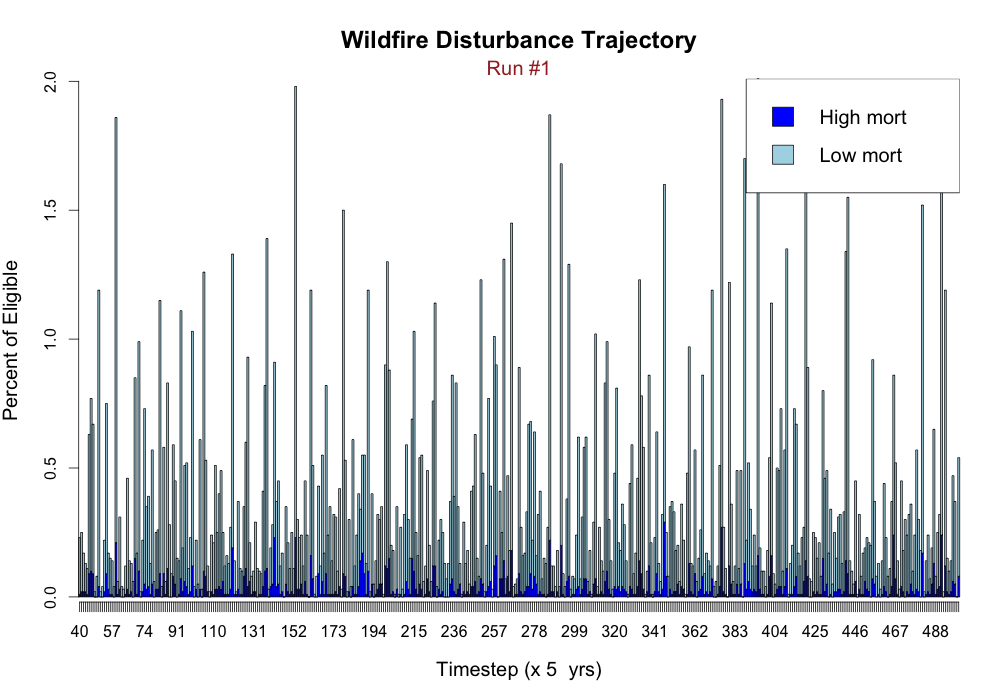
\includegraphics[width=0.48\textwidth]{/Users/mmallek/Tahoe/Report2/images/darea_megm.png}
    \caption{Disturbance trajectory for Mixed Evergreen - Mesic. High mortality fire in dark blue; low mortality fire in light blue.}
	\label{fig:darea_megm}
\end{wrapfigure}

Mixed Evergreen - Mesic (\textsc{meg\_m})is a somewhat common cover type within the core project area, encompassing 7,273 ha and comprising roughly 4\% of the project area. The frequency and extent of simulated wildfires in cool moist mixed-conifer forest varied markedly among decades (Figure \ref{fig:darea_megm} and Table \ref{tab:darea_megm}). While \textsc{meg\_m} escaped fire completely five times during the simulation, during a typical five year period a small portion of the cover type burned, mostly with a low mortality effect. Seldom did large extents of \textsc{meg\_m} burn, at any mortality level, although roughly once every 60 years, $>25\%$ of the cover type burned. 

Under this wildfire regime, the return interval between fires (of any mortality level) varied widely from X to X years, with a mean and median of X and X years, respectively. As expected, return intervals varied spatially across the forest (Figure \ref{fig:preturn_megm}). In general, return intervals increased with increasing TPI, reflecting the moister, cooler conditions at higher elevations. In addition, \textsc{meg\_m} stands embedded in a neighborhood containing cover types with shorter return intervals exhibited shorter return intervals, reflecting the importance of landscape context on fire regimes.

\todo{next! age structure}


\begin{table}[!htbp]
\centering
\caption{Disturbed area summary statistics for Mixed Evergreen - Mesic. Proportions shown are relative to the total area of Mixed Evergreen - Mesic.}
\label{tab:darea_megm}
	\begin{tabular}{@{}llll@{}} 
	\toprule
	\textbf{\begin{tabular}[c]{@{}l@{}}Summary Statistic \\ (disturbed area/timestep)\end{tabular}} & \textbf{\begin{tabular}[c]{@{}l@{}}Low  Mortality\end{tabular}} & \textbf{\begin{tabular}[c]{@{}l@{}}High  Mortality\end{tabular}} & \textbf{\begin{tabular}[c]{@{}l@{}}Any  Mortality\end{tabular}} \\ \midrule
	Minimum       & 0.00        &  0.00         & 0.00         \\
	Maximum       & 46.18       & 7.24          & 50.17         \\
	Median        & 4.99        &  0.50         & 5.99         \\
	Mean          & 8.24        &  1.00         & 9.24         \\ \bottomrule
	\end{tabular}
\end{table}

%\begin{wrapfigure}{r}{0.5\textwidth}
%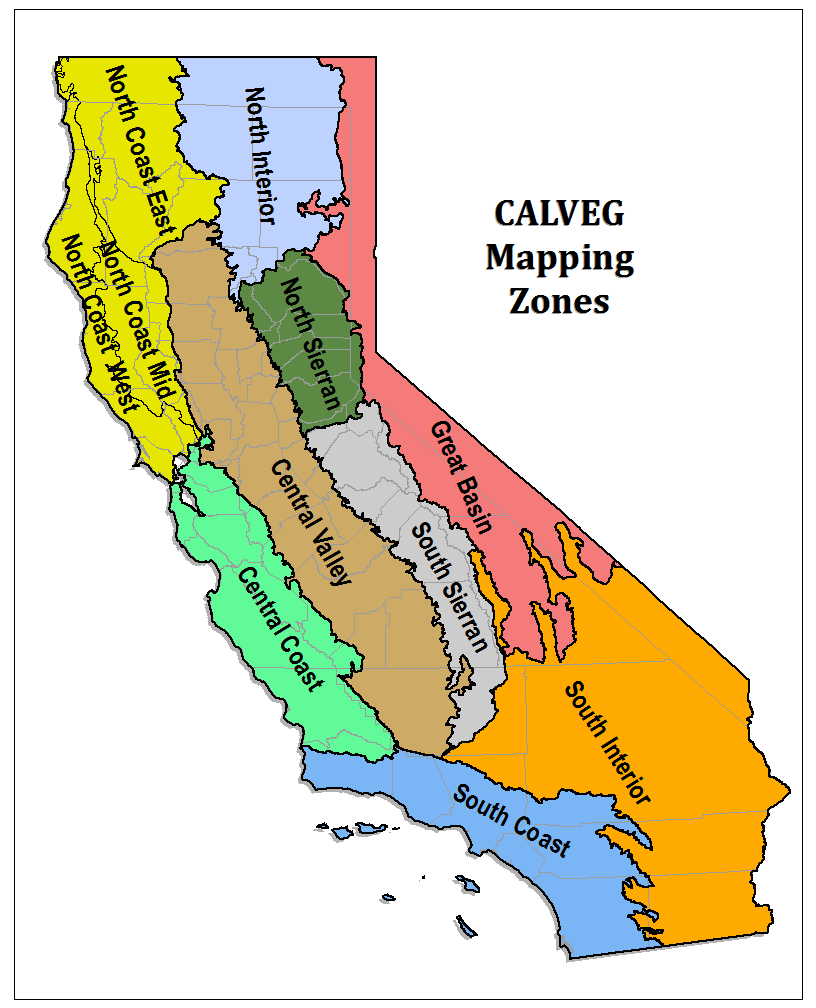
\includegraphics[width=0.48\textwidth]{images/CALVEGmappingzones.png}
%\caption{\small CALVEG Mapping Zones. These zones meet U.S. Forest Service standard at national and regional levels. These ecological provinces are %associated with dozens of vegetation alliances, which are used to classify vegetation in spatial data products.} 
%\label{calveg}
%\end{wrapfigure}

\subsection{Mixed Evergreen - Xeric} 

\begin{table}[!htbp]
\centering
\caption{Disturbed area summary statistics for Mixed Evergreen - Xeric. Proportions shown are relative to the total area of Mixed Evergreen - Xeric.}
\label{tab:darea_megx}
\begin{tabular}{@{}llll@{}}
\toprule
\textbf{\begin{tabular}[c]{@{}l@{}}Summary Statistic \\ (disturbed area/timestep)\end{tabular}} & \textbf{Low Mortality} & \textbf{High Mortality} & \textbf{Any Mortality} \\ \midrule
Minimum       & 0.00	& 	0.00	& 0.00        \\
Maximum       & 54.72	& 	8.58	& 58.48         \\
Median        & 6.97	& 	0.54	& 7.78        \\
Mean          & 10.19	& 	1.07	& 11.27        \\ \bottomrule
\end{tabular}
\end{table}


\subsection{Oak-Conifer Forest and Woodland} 

\begin{table}[!htbp]
\centering
\caption{Disturbed area summary statistics for Oak-Conifer Forest and Woodland. Proportions shown are relative to the total area of Oak-Conifer Forest and Woodland.}
\label{tab:darea_ocfw}
\begin{tabular}{@{}llll@{}}
\toprule
\textbf{\begin{tabular}[c]{@{}l@{}}Summary Statistic \\ (disturbed area/timestep)\end{tabular}} & \textbf{Low Mortality} & \textbf{High Mortality} & \textbf{Any Mortality} \\ \midrule
Minimum       & 0.39	& 0.00	& 0.47       \\
Maximum       & 59.90	& 22.77	& 81.34         \\
Median        & 11.93	& 3.82	& 16.22       \\
Mean          & 15.75	& 5.23	& 20.90        \\ \bottomrule
\end{tabular}
\end{table}



\subsection{Oak-Conifer Forest and Woodland - Ultramafic} 

\begin{table}[!htbp]
\centering
\caption{Disturbed area summary statistics for Oak-Conifer Forest and Woodland - Ultramafic. Proportions shown are relative to the total area of Oak-Conifer Forest and Woodland - Ultramafic.}
\label{tab:darea_ocfwu}
\begin{tabular}{@{}llll@{}}
\toprule
\textbf{\begin{tabular}[c]{@{}l@{}}Summary Statistic \\ (disturbed area/timestep)\end{tabular}} & \textbf{Low Mortality} & \textbf{High Mortality} & \textbf{Any Mortality} \\ \midrule
Minimum       & 0.00	&   0.00	& 0.00       \\
Maximum       & 83.93	&   5.14	& 85.64         \\
Median        & 5.14	&   0.00	& 5.14       \\
Mean          & 10.28	&   0.00	& 10.28        \\ \bottomrule
\end{tabular}
\end{table}



\subsection{Red Fir - Mesic} 

\begin{table}[!htbp]
\centering
\caption{Disturbed area summary statistics for Red Fir - Mesic. Proportions shown are relative to the total area of Red Fir - Mesic.}
\label{tab:darea_rfrm}
\begin{tabular}{@{}llll@{}}
\toprule
\textbf{\begin{tabular}[c]{@{}l@{}}Summary Statistic \\ (disturbed area/timestep)\end{tabular}} & \textbf{Low Mortality} & \textbf{High Mortality} & \textbf{Any Mortality} \\ \midrule
Minimum       & 0.00	& 	0.00	& 0.00        \\
Maximum       & 54.72	& 	8.58	& 58.48         \\
Median        & 6.97	& 	0.54	& 7.78        \\
Mean          & 10.19	& 	1.07	& 11.27        \\ \bottomrule
\end{tabular}
\end{table}



\subsection{Red Fir - Xeric} 

\begin{table}[!htbp]
\centering
\caption{Disturbed area summary statistics for Red Fir - Xeric. Proportions shown are relative to the total area of Red Fir - Xeric.}
\label{tab:darea_rfrx}
\begin{tabular}{@{}llll@{}}
\toprule
\textbf{\begin{tabular}[c]{@{}l@{}}Summary Statistic \\ (disturbed area/timestep)\end{tabular}} & \textbf{Low Mortality} & \textbf{High Mortality} & \textbf{Any Mortality} \\ \midrule
Minimum       & 0.00	& 	0.00	& 0.00     \\
Maximum       & 54.52	& 	32.71	& 80.68        \\
Median        & 4.60	& 	2.18	& 6.78     \\
Mean          & 8.72	& 	4.36	& 13.33      \\ \bottomrule
\end{tabular}
\end{table}



\subsection{Sierran Mixed Conifer - Mesic} 

\begin{table}[!htbp]
\centering
\caption{Disturbed area summary statistics for Sierran Mixed Conifer - Mesic. Proportions shown are relative to the total area of Sierran Mixed Conifer - Mesic.}
\label{tab:darea_smcm}
\begin{tabular}{@{}llll@{}}
\toprule
\textbf{\begin{tabular}[c]{@{}l@{}}Summary Statistic \\ (disturbed area/timestep)\end{tabular}} & \textbf{Low Mortality} & \textbf{High Mortality} & \textbf{Any Mortality} \\ \midrule
Minimum       & 0.19	& 	0.03	& 0.22       \\
Maximum       & 51.09	& 	24.42	& 74.53         \\
Median        & 10.54	& 	3.36	& 13.90       \\
Mean          & 13.46	& 	4.52	& 17.98        \\ \bottomrule
\end{tabular}
\end{table}



\subsection{Sierran Mixed Conifer - Ultramafic} 

\begin{table}[!htbp]
\centering
\caption{Disturbed area summary statistics for Sierran Mixed Conifer - Ultramafic. Proportions shown are relative to the total area of Sierran Mixed Conifer - Ultramafic.}
\label{tab:darea_smcu}
\begin{tabular}{@{}llll@{}}
\toprule
\textbf{\begin{tabular}[c]{@{}l@{}}Summary Statistic \\ (disturbed area/timestep)\end{tabular}} & \textbf{Low Mortality} & \textbf{High Mortality} & \textbf{Any Mortality} \\ \midrule
Minimum       & 0.00	& 0.00		& 0.00      \\
Maximum       & 32.14	& 21.13		& 52.83        \\
Median        & 2.64	& 1.32		& 4.40      \\
Mean          & 4.84	& 2.64		& 7.48       \\ \bottomrule
\end{tabular}
\end{table}



\subsection{Sierran Mixed Conifer - Xeric} 

\begin{table}[!htbp]
\centering
\caption{Disturbed area summary statistics for Sierran Mixed Conifer - Xeric. Proportions shown are relative to the total area of Sierran Mixed Conifer - Xeric.}
\label{tab:darea_smcx}
\begin{tabular}{@{}llll@{}}
\toprule
\textbf{\begin{tabular}[c]{@{}l@{}}Summary Statistic \\ (disturbed area/timestep)\end{tabular}} & \textbf{Low Mortality} & \textbf{High Mortality} & \textbf{Any Mortality} \\ \midrule
Minimum       & 0.28	& 0.03	  & 0.38    \\
Maximum       & 52.00	& 35.55	  & 84.90       \\
Median        & 9.98	& 6.26	  & 16.80    \\
Mean          & 12.83	& 8.42	  & 21.25     \\ \bottomrule
\end{tabular}
\end{table}






\section{Overall Landscape Assessment}

First, we note that during the HRV, the landscape was composed of larger and more extensive patches, as illustrated by Figure \ref{fig:fragland_areashape}. 
Second, patches on the landscape were more aggregated at the cell-level during HRV, which is illustrated by the \emph{Contagion} metric. In addition, we observe increased dominance by certain cover types, as illustrated by smaller values for the \emph{Simpson's Evenness Index} durin the HRV (see Figure \ref{fig:fragland_contagsiei}). However, despite being larger, more extensive, and aggregated, they do not show an associated increase in core area. This indicates that they are geometrically more complex, to the extent that little core area fits inside each patch. As an example, we highlight in Figure \ref{fig:fragland_core} a patch of Sierran Mixed Conifer - Mesic Forest in the Mid Development - Closed condition, which is one of the largest patches on the landscape. Little room is available for cores due to the irregular shape of this patch.
